\section{Runtime and causal service}
\label{sec:runtime}

The deployment measurements in this article use persistent services: weights remain resident, state advances with causal sensor arrivals, and previously computed work is reused when its inputs are unchanged. PHASE and Garl receive the same paced RAW replay. The primary response clock begins at scheduled arrival and ends when the required TTC output is available on the host. It includes sensor release, scheduling and queueing, region preparation, neural computation, synchronization, and delivery. Model loading, synthetic shape priming, history initialization, and RAW disk preload occur before measured arrivals. This is a CPU-fed sensor replay, not a physical-camera measurement.

\begin{figure}[H]
\centering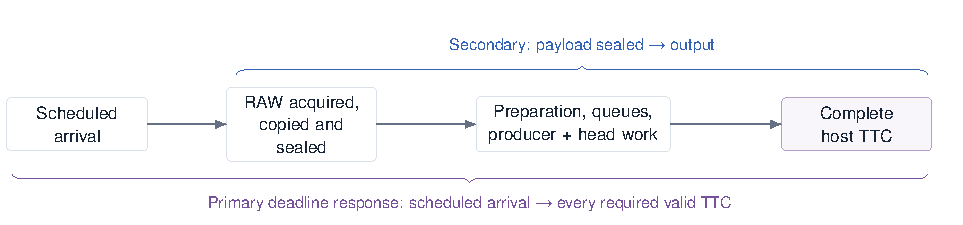
\includegraphics[width=\linewidth]{figures/publication_runtime_clock.pdf}
\caption{\textbf{Persistent-service response clocks.} The primary clock starts at scheduled arrival. The secondary clock starts after RAW acquisition, copy, and payload sealing. Both end at completed host TTC output. Service time starts only when the consumer begins work and is reported separately.}
\label{fig:runtime-clocks}
\end{figure}

\subsection{Persistent execution and exact reuse}

PHASE prepares RGB within the object region, extends event prefixes incrementally, and reuses reverse-transport summaries exactly. Top-$k$ normalization and native query graphs reduce repeated work; parallel branches overlap event execution with RGB preparation. Previously computed RGB producer features are reused under matching identities, while event encodings and temporal readouts are recomputed. Native numerical agreement is checked separately for the complete output chain. The complete nine-component model is retained.

The comparator is persistent TTC-only Garl. Its weights and causal event history remain resident; exact endpoint representations and the six-channel paired RGB backbone result are reused only under matching sensor, geometry, model, and preprocessing identities. Its event backbone and TTC heads execute on every completed update. Auxiliary foreground decoders are disabled because their masks do not feed the TTC output. All raw heights and TTC predictions are verified against untouched native inference after timing; the complete checkpoint remains loaded.

Compiled transport alternatives that changed PHASE's TTC on sensitive examples were rejected. An earlier smaller-packet experiment established numerical equivalence but did not establish paced-service latency. Neither result is substituted for the measured production-service response. \evidence{L41,L42}

\subsection{Expanded repeated inference study}

The subsequent campaign extends the comparison to six recorded car and pedestrian scenarios, using 1,979 distinct sensor-clock anchors and continuous intervals up to 9.3\,s. It retains 72 fresh-process attempts: four repetitions per model and scenario with queue capacity two, and two additional repetitions with queue capacity 64. All timing finishes before independent native-reference inference begins, and both services apply a fixed rest after initialization. This separates the expanded evidence from the initial experiment's interleaved reference workload.

\begin{table}[H]
\centering\small
\caption{\textbf{Expanded persistent-service comparison at 50\,Hz.} S1--S6 denote CPLA-low, CCRm-medium-0, CCRs-3-low-100, CCRs-side-high, CPNA-high and CPNAO-high. Q2 and Q64 denote queue capacities two and 64. D/A/N gives complete deliveries, numerically admitted runs and declared attempts. Median per-pass p95 (ms) requires full delivery and native parity in all four Q2 repetitions or both Q64 repetitions; all attempts remain in the full tables.}
\begin{tabular}{llrrrr}
\toprule
Scene & Model & Q2 D/A/N & Q2 p95 & Q64 D/A/N & Q64 p95 \\
\midrule
S1 & PHASE & 0/0/4 & --- & 2/2/2 & 121.66 \\
S1 & Garl & 0/0/4 & --- & 2/2/2 & 2932.78 \\
S2 & PHASE & 0/0/4 & --- & 2/0/2 & --- \\
S2 & Garl & 0/0/4 & --- & 2/2/2 & 1741.70 \\
S3 & PHASE & 1/1/4 & --- & 2/2/2 & 105.15 \\
S3 & Garl & 0/0/4 & --- & 0/0/2 & --- \\
S4 & PHASE & 0/0/4 & --- & 2/2/2 & 226.71 \\
S4 & Garl & 0/0/4 & --- & 0/0/2 & --- \\
S5 & PHASE & 0/0/4 & --- & 2/2/2 & 175.53 \\
S5 & Garl & 0/0/4 & --- & 2/2/2 & 4934.71 \\
S6 & PHASE & 0/0/4 & --- & 2/2/2 & 103.72 \\
S6 & Garl & 0/0/4 & --- & 1/1/2 & --- \\
\bottomrule
\end{tabular}

\end{table}

With the two-packet queue, PHASE completed 1/24 full replays and delivered 762/7,916 outputs (9.6\%). Of all offered updates, 178 (2.2\%) completed below 20\,ms. Strict native parity admitted 1/24 full replays; 0 delivered outputs failed at least one required numerical check.

With the two-packet queue, Garl completed 0/24 full replays and delivered 72/7,916 outputs (0.9\%). Of all offered updates, 0 (0.0\%) completed below 20\,ms. Strict native parity admitted 0/24 full replays; 0 delivered outputs failed at least one required numerical check.

With the 64-packet queue, PHASE completed 12/12 full replays and delivered 3,958/3,958 outputs (100.0\%). Of all offered updates, 1,217 (30.7\%) completed below 20\,ms. Strict native parity admitted 10/12 full replays; 6 delivered outputs failed at least one required numerical check.

With the 64-packet queue, Garl completed 7/12 full replays and delivered 3,816/3,958 outputs (96.4\%). Of all offered updates, 429 (10.8\%) completed below 20\,ms. Strict native parity admitted 7/12 full replays; 0 delivered outputs failed at least one required numerical check.

Appendix~\ref{sec:extended-inference} reports cohort selection, complete architecture and execution contracts, per-pass distributions, service and queue clocks, deadline coverage, buffered response traces, memory, startup, source age and independent numerical verification. A larger queue can preserve more packets while increasing the age of delivered TTC; those diagnostic results are kept separate from the two-packet primary policy.

\subsection{Historical persistent-service reference}

The initial three-pass matched comparison did not establish complete repeated-service coverage. Its native-oracle work was interleaved with subsequent timing without a controlled rest, so it remains a separate historical experiment. Appendix~\ref{sec:local-hardware} retains every pass, including failures and the earlier eager-Garl control.

The earlier five-second replay completed all 250 updates with numerical parity, zero drops and zero source errors. Its scheduled-arrival latency was 29.14\,ms at p95, 32.41\,ms at p99, and 35.33\,ms at maximum. Of the 250 responses, 201 reached or exceeded 20\,ms. Starting the clock after RAW acquisition, copy and payload sealing gave a p95 of 25.25\,ms. This remains a historical single-run reference, distinct from the contemporaneous repeated comparison above. \evidence{L40,R02}

\begin{figure}[t]
\centering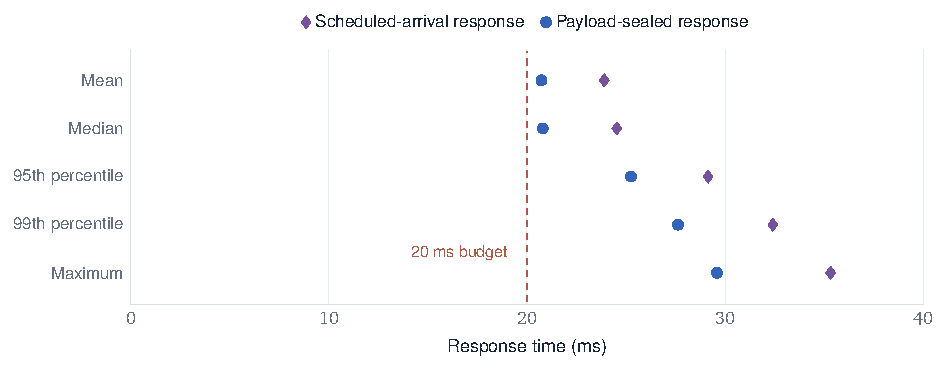
\includegraphics[width=0.98\linewidth]{figures/publication_runtime.pdf}
\caption{\textbf{Historical persistent PHASE reference.} The original 250-update replay has scheduled-arrival p95 29.14\,ms; 201 responses reach or exceed 20\,ms. This figure is not a new Garl comparison. \evidence{L40}}
\end{figure}

All deployment measurements here exclude disk I/O and cover one supplied object region. The initial comparison uses five-second replays; the expanded campaign uses distinct continuous intervals of 3.1--9.3\,s. Neither establishes physical-camera operation, upstream object detection, sixty-second sustained service, multi-object capacity, or calibrated safety decisions. Earlier query-oriented adapter experiments remain in the evidence archive, but their timings are excluded from this article's deployment-latency comparison.
\FloatBarrier
